%!TEX encoding = UTF-8 Unicode
%!TEX root = ../lect-w10.tex

%%%


%\begin{Slide}{TODO: Begrepp att förklara}
%  Tänk igenom ordningen:
%  \begin{itemize}
%    \item OO, arv, supertyp, subtyp, bastyp, polymorfism, ...
%  \end{itemize}
%\end{Slide}


\Subsection{Överskuggingsregler, \texttt{override}}

\begin{Slide}{Medlemmar, arv och överskuggning}\SlideFontTiny
\begin{multicols}{2}
\noindent Olika sorters överskuggningsbara medlemmar i \Emph{Scala}:
\begin{itemize}
\item \code{def}
\item \code{val}
\item \code{lazy val}
\item \code{var}
\end{itemize}


\columnbreak

\pause

\noindent Olika sorters överskuggningsbara instansmedlemmar i \Emph{Java}:
\begin{itemize}
\item variabel
\item metod
\end{itemize}

{\SlideFontTiny\noindent Medlemmar som är \jcode{static} kan ej överskuggas (men döljas) vid arv.}

\vspace{0.5em}
\end{multicols}

\pause
\begin{itemize}\SlideFontTiny
\item När man överskuggar \Eng{override} en medlemmen med en annan medlem med samma namn i en subtyp, får denna medlem en (ny) implementation.

\item När man konstruerar ett objektorienterat språk gäller det att man definierar sunda överskuggningsregler vid arv. Detta är förvånansvärt knepigt.

\item Singelobjekt kan ej ärvas (och medlemmar i singelobjekt kan därmed ej överskuggas).
\end{itemize}
\end{Slide}


\begin{Slide}{Fördjupning: Regler för överskuggning i Scala} \SlideFontTiny
\label{slideW07:overriderules}
En medlem M1 i en supertyp får överskuggas av en medlem M2 i en subtyp, enligt dessa regler:
\begin{enumerate}
\item M1 och M2 ska ha samma namn och typerna ska matcha.
\item \code{def} får bytas ut mot: \code{def}, \code{val}, \code{var}, \code{lazy val}
\item \code{val} får bytas ut mot: \code{val}, och om M1 är abstrakt mot en \code{lazy val}.
\item \code{var} får bara bytas ut mot en \code{var}.
\item \code{lazy val} får bara bytas ut mot en \code{lazy val}.
\item Om en medlem i en supertyp är abstrakt \emph{behöver} man inte använda nyckelordet \code{override} i subtypen. (Men det är bra att göra det ändå så att kompilatorn hjälper dig att kolla att du verkligen överskuggar något.)
\item Om en medlem i en supertyp är konkret \emph{måste} man använda nyckelordet \code{override} i subtypen, annars ges kompileringsfel.
\item M1 får inte vara \code{final}.
\item M1 får inte vara \code{private} eller \code{private[this]}, men kan vara \code{private[X]} om M2 också är \code{private[X]}, eller \code{private[Y]} om X innehåller Y.
\item Om M1 är \code{protected} måste även M2 vara det.

\end{enumerate}
\end{Slide}


\Subsection{\texttt{super}}

\begin{Slide}{Att skilja på mitt och ditt med \texttt{super}}
\begin{REPL}
scala> class X { def gurka = "super pepino" }

scala> class Y extends X {
         override val gurka = ":("
         val sg = super.gurka
       }

scala> val y = new Y
y: Y = Y@26ba2a48

scala> y.gurka
res0: String = :(
\end{REPL}

\pause
Super Pepinos to the rescue:
\begin{REPLnonum}
scala> y.sg
res1: String = super pepino

\end{REPLnonum}


\pause
\begin{tikzpicture}[overlay]
     \node at (7.5,1.7) {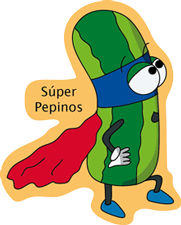
\includegraphics[scale=0.5]{../img/ttsuper}};
\end{tikzpicture}
\href{https://youtu.be/NPhjiXskz34}{\small https://youtu.be/NPhjiXskz34}
%\href{http://www.pepinadas.com/}{\small www.pepinadas.com/}
\end{Slide}



\begin{Slide}{Terminologi och nyckelord vid arv}\SlideFontTiny

\begin{tabular}{r  l}
\Emph{subtyp}           & en typ som ärver en supertyp\\
\Emph{supertyp}         & en typ som ärvs av en subtyp\\
\Emph{bastyp}           & en typ som är rot i ett arvsträd\\
\Emph{abstrakt medlem}  & en medlem som saknar implementation\\
\Emph{konkret medlem}   & en medlem som ej saknar implementation\\
\Emph{abstrakt typ}     & en typ som kan ha abstrakta medlemmar; kan ej instansieras\\
\Emph{konkret typ}      & en typ som ej har abstrakta medlemmar; kan instansieras\\
\code|class|            & en konkret typ som \Alert{kan ej ha abstrakta medlemmar}\\
\code|abstract class|   & en abstrakt typ som \Emph{kan ha abstrakta medlemmar}\\
\code|trait|            & är en abstrakt typ som \Emph{kan mixas in} \\
\code|extends|          & står före en supertyp, medför arv av supertypens medlemmar\\
\code|override|         & en medlem överskuggar (byter ut) en medlem i en superttyp\\
\code|protected|        & gör en medlem synlig i subtyper till denna typ (jmf \code|private|)\\
\code|final gurka|      & gör medlemen gurka final: förhindrar överskuggning\\
\code|final class|      & gör klassen final: förhindrar vidare subtypning\\
\code|sealed|           & förseglad trait/klass: enbart subtyper i denna kodfil, koll av match\\
\code|open class|       & berätta att den är tänkt att ärvas, \code|open| krävs för arv i annan kodfil\\   
\code|transparent trait|& gör typen osynlig vid typhärledning\\
\code|super.gurka|      & refererar till supertypens medlem \code|gurka| (jmf \code|this|)\\

\end{tabular}

\ifkompendium\else
\pause
\begin{tikzpicture}[overlay]
     \node at (10.7,0.6) {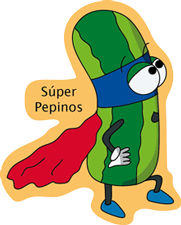
\includegraphics[scale=0.36]{../img/ttsuper}};
\end{tikzpicture}
\fi

\end{Slide}



\Subsection{Algebraiska datatyper}

\begin{Slide}{Terminologi för datatyper}\SlideFontSmall
\begin{itemize}
\item Abstrakt datatyp \Eng{abstract data type}
\begin{itemize}\SlideFontTiny
\item Definieras av gränssnittet och beteendet -- implementationen är dold för användaren. 
\item Fördelar: inkapsling, lokala ändringar, flexibilitet.
\item Skapas i Scala t.ex. med klasser + privata medlemmar.
\end{itemize} 
\item Enumeration, ä.k. uppräkning \Eng{enumeration}
\begin{itemize}\SlideFontTiny
\item En speciellt enkel form av s.k. algebraisk datatyp som består av en uppräknad, ändlig sekvens av enkla värden som har en ordning.
\item Skapas i Scala med 1) heltal, 2) \code{sealed trait} ... \code{case class} ... 3) \code{enum}
\end{itemize} 
\item Algebraisk datatyp \Eng{algebraic data type}
\begin{itemize}\SlideFontTiny
\item En datatyp som är sammansatt av delar som kan kombineras. 
\item Två olika algebraiska datatyper som kan kombineras med varandra:
\begin{itemize}\SlideFontTiny
\item \Alert{Och}-typ (ä.k. produkttyp, record, struct), exempel: \\ \code|case class Person(namn: Int, ålder: Int)| \\består av attributen namn \Alert{OCH} ålder.
\item \Emph{Eller}-typ (ä.k. summatyp), exempel: \code|enum Färg { case Röd, Svart}| \\kan vara antingen röd \Emph{ELLER} svart.
\end{itemize}  
\end{itemize} 
\end{itemize}     
\end{Slide}


\begin{Slide}{Algebraiska datatyper}
     \TODO visa med både case classer och enum
\end{Slide}

\begin{Slide}{Typunioner med eller-operator}
     \TODO
\end{Slide}